\documentclass[letterpaper, 12pt]{article}
\usepackage{comment} % enables the use of multi-line comments (\ifx \fi) 
\usepackage{fullpage} % changes the margin
\usepackage[T1]{fontenc}
\usepackage{selinput}
\usepackage{enumitem}
\usepackage{listings}
\usepackage{amsmath}
\usepackage{amssymb}
\usepackage{amsthm}
\usepackage{setspace}
\usepackage{bm}
\usepackage{mathtools}
\usepackage{tikz}
\usepackage{xcolor}

\renewcommand\qedsymbol{$\blacksquare$}
\newtheorem{theorem}{Theorem}
\newtheorem{corollary}{Corollary}[theorem]
\newtheorem{lemma}[theorem]{Lemma}
\newtheorem{definition}[theorem]{Definition}

\begin{document}
\noindent
\large\textbf{"Cattle Land"} \hfill \textbf{Quinn Murphey} \\
\normalsize \hfill Date: 03/13/19 \\
\noindent\makebox[\linewidth]{\rule{\paperwidth}{0.4pt}}

\section*{Problem}

\textit{Given an $n\times m$ lattice where $n\geq m$, how many unique monotonically increasing (only moving Right or Up) paths from $(0,0)$ to the point $(n,m)$ which do not pass above the line defined by $y=x$.} Figure \ref{fig:Example} shows an example path which follows this criterion on a $5\times5$ lattice.

\begin{figure}[h]
    \centering
    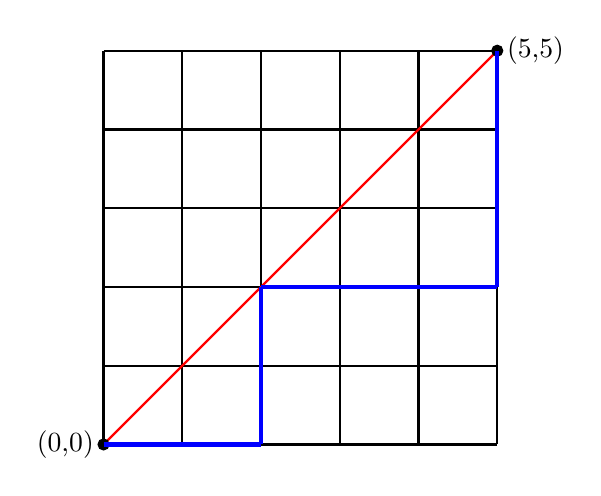
\begin{tikzpicture}
        \draw[black, thick] (0,0) -- (5,0);
        \draw[black, thick] (0,1) -- (5,1);
        \draw[black, thick] (0,2) -- (5,2);
        \draw[black, thick] (0,3) -- (5,3);
        \draw[black, thick] (0,4) -- (5,4);
        \draw[black, thick] (0,5) -- (5,5);
        \draw[black, thick] (0,0) -- (0,5);
        \draw[black, thick] (1,0) -- (1,5);
        \draw[black, thick] (2,0) -- (2,5);
        \draw[black, thick] (3,0) -- (3,5);
        \draw[black, thick] (4,0) -- (4,5);
        \draw[black, thick] (5,0) -- (5,5);
        \draw[red, thick] (0,0) -- (5,5);
        \filldraw[black] (0,0) circle (2pt) node[anchor=east] {(0,0)};
        \filldraw[black] (5,5) circle (2pt) node[anchor=west] {(5,5)};
        \draw[blue, ultra thick] (0,0) -- (2,0);
        \draw[blue, ultra thick] (2,0) -- (2,2);
        \draw[blue, ultra thick] (2,2) -- (5,2);
        \draw[blue, ultra thick] (5,2) -- (5,5);
    \end{tikzpicture}
    \caption{A 5$\times$5 lattice with $y=x$ in red and a valid path in blue}
    \label{fig:Example}
\end{figure}
\section*{Solution}
Since the basis $\{(1,0),(0,1)\}$ spans the entire lattice by addition (or positive integer multiplication). We represent each point $n(1,0) + m(0,1)$ as $(n,m)$.
\begin{lemma}\label{lem:totalPaths}
Given two positive integers $n$ and $m$, there are 
\begin{equation*}
    \binom{n+m}{n} \quad = \quad \frac{(n+m)!}{(n)!(m)!}
\end{equation*}
unique monotonically increasing paths originating at $(0,0)$ which end at $(n,m)$.
\end{lemma}
\begin{proof}
Since each path is monotonically increasing, it takes $n$ rightward steps and $m$ upward steps to reach $(n,m)$. Therefore we have $(n+m)!$ path representations. Since we can order the $n$ right steps $n!$ ways and the $m$ up steps $m!$ ways. Each path has $(n)!(m)!$ representations so the total number of unique paths is 
\begin{align*}
    \frac{(n+m)!}{(n)!(m)!} 
    =\binom{n+m}{n}.
\end{align*}
\end{proof}
\begin{definition}
We will call any path that passes above the line $y=x$ at least once a bad path and any path that is not a bad path a good path. Unless otherwise stated, every path will start at the origin: $(0,0)$.
\end{definition}
Since any path which passes above the line $y=x$ is a bad path by definition, we can will disregard all paths which move up first and only include paths which move right first. This changes our origin to $(1,0)$ or shifts each path to the right 1 and changes the number of paths to each $(n,m)$ to 
\begin{equation}\label{eq:modifiedTotal}
    \binom{n+m-1}{n-1}.
\end{equation}
\begin{lemma}\label{lem:goodPathEq}
    The number of good paths from the origin to $(n,m)$ is equal to the total number of paths to $(n,m)$ minus the number of bad paths to $(n,m)$.
\end{lemma}
\begin{proof}
    Let $P$ be the set of all paths from $(0,0)$ to $(n,m)$ and $p=\#(P)$, let $B$ be the set of all bad paths from $(0,0)$ to $(n,m)$ and $b=\#(B)$, and let $G$ be the set of all good paths from $(0,0)$ to $(n,m)$ and $g=\#(G)$. $G$ and $B$ are obviously subsets of $P$ which means that $G = B^c = P\setminus B$ by definition of a good path. This also means that $g = p-b$ concluding our proof. 
\end{proof}

Now instead of finding the number of good paths to $(n,m)$ directly we just need to find the total number of paths and the number of bad paths to $(n,m)$.
\begin{definition}
An alternate definition for a bad path is a path which touches the line $y=x+1$ at least once. Also, we will call this line the fatal line. The definition for good path is still a path which is not bad.
\end{definition}
This is equivalent because every line that passes above the line $y=x$ immediately touches the fatal line due to us only considering paths which start below $y=x$, more specifically at $(0,0)$. (See Figure \ref{fig:fatalLine})\\

In order to complete the proof we must show the following:
\begin{lemma}\label{lem:extendLattice}
    The set of paths from $(0,0)$ to $(n,m)$ is invariant to increasing the size of the overall lattice in which these points reside.
\end{lemma}
\begin{proof}
    Since each path is monotonic, it can only move away from the origin the in positive x and y direction. Therefore you can only strictly increase along the ranks shown in Figure \ref{fig:ranks}. The ranks also show how many steps it takes to reach any given point along that rank. Since moving left or moving down would be decreasing the path's rank we cannot do that. Therefore, since having a larger lattice only adds points to the right and above any points in our original lattice, there exist no paths which pass through any new points as well as $(n,m)$. Therefore, since no possible paths were removed either, the set of paths remains the same as if it were on a $n\times m$ lattice.
\end{proof}
\newpage
\begin{figure}[t]
    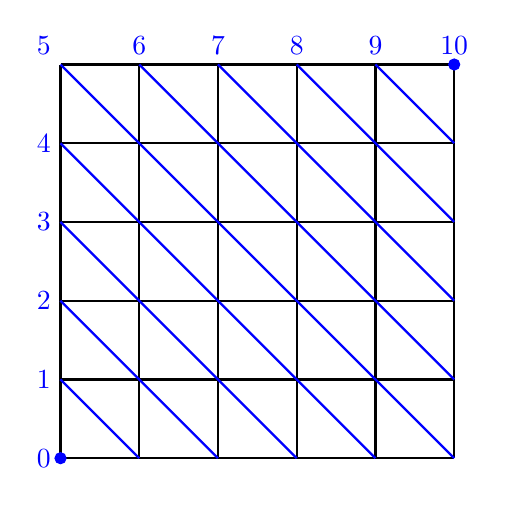
\begin{tikzpicture}
        \draw[black, thick] (0,0) -- (5,0);
        \draw[black, thick] (0,1) -- (5,1);
        \draw[black, thick] (0,2) -- (5,2);
        \draw[black, thick] (0,3) -- (5,3);
        \draw[black, thick] (0,4) -- (5,4);
        \draw[black, thick] (0,5) -- (5,5);
        \draw[black, thick] (0,0) -- (0,5);
        \draw[black, thick] (1,0) -- (1,5);
        \draw[black, thick] (2,0) -- (2,5);
        \draw[black, thick] (3,0) -- (3,5);
        \draw[black, thick] (4,0) -- (4,5);
        \draw[black, thick] (5,0) -- (5,5);
        
        \draw[blue, thick] (0,1) -- (1,0);
        \draw[blue, thick] (0,2) -- (2,0);
        \draw[blue, thick] (0,3) -- (3,0);
        \draw[blue, thick] (0,4) -- (4,0);
        \draw[blue, thick] (0,5) -- (5,0);
        \draw[blue, thick] (1,5) -- (5,1);
        \draw[blue, thick] (2,5) -- (5,2);
        \draw[blue, thick] (3,5) -- (5,3);
        \draw[blue, thick] (4,5) -- (5,4);
        
        \filldraw[blue] (0,0) circle (2pt) node[anchor=east] {0};
        \filldraw[blue] (0,1) circle (0pt) node[anchor=east] {1};
        \filldraw[blue] (0,2) circle (0pt) node[anchor=east] {2};
        \filldraw[blue] (0,3) circle (0pt) node[anchor=east] {3};
        \filldraw[blue] (0,4) circle (0pt) node[anchor=east] {4};
        \filldraw[blue] (0,5) circle (0pt) node[anchor=south east] {5};
        \filldraw[blue] (1,5) circle (0pt) node[anchor=south] {6};
        \filldraw[blue] (2,5) circle (0pt) node[anchor=south] {7};
        \filldraw[blue] (3,5) circle (0pt) node[anchor=south] {8};
        \filldraw[blue] (4,5) circle (0pt) node[anchor=south] {9};
        \filldraw[blue] (5,5) circle (2pt) node[anchor=south] {10};
    \end{tikzpicture}
    \centering
    \caption{"Ranks" are shown and labeled in blue}
    \label{fig:ranks}
\end{figure}

\begin{lemma}\label{lem:badPathEq}
    The number of bad paths from $(1,0)$ to $(n,m)$ is equal to the number of paths from $(1,0)$ to $(m-1,n+1)$ which is $$\binom{n+m-1}{n+1}$$
\end{lemma}
\begin{proof}
    Let $s=n+1$. We will extend our lattice to a $s\times s$ lattice. Due to Lemma \ref{lem:extendLattice}, this does not change the set of paths from $(0,0)$ to $(n,m)$. Every bad path touches the fatal line at least once. Therefore, due to the monotonicity of the paths, the bad paths (excluding the path before it touches the fatal line) are symmetric across the fatal line. Since the paths themselves are symmetric across the fatal line, the number of paths going to each point on the lattice is also symmetric across the fatal line. Therefore the number of bad paths from $(1,0)$ to $(n,m)$ is the same as the number of bad paths going to $(m-1,n+1)$ (which is on our extended lattice), the reflection of $(n,m)$ across the fatal line ($y=x+1$). Since $n\geq m$, $m-1 < n+1$ which means that $(m-1,n+1)$ is strictly above the line $y=x$. Therefore every path from $(1,0)$ to $(m-1,n+1)$ is a bad path. So the set of all bad paths to $(m-1,n+1)$ is equal to the set of all paths from $(1,0)$ to $(m-1,n+1)$. Which then implies that the number of paths from $(1,0)$ to $(m-1,n+1)$ is equal to the number of bad paths from $(1,0)$ to $(n,m)$. The number of paths from $(1,0)$ to $(m-1,n+1)$ equals
    \begin{align*}
        \binom{n+m-1}{m-1} = \binom{n+m-1}{n+1}
    \end{align*}
\end{proof}
See Figure \ref{fig:countingPaths} for an example of the symmetry and the number of paths from (1,0) to each point on a $5\times5$ lattice.
\newpage
\begin{figure}[t]
    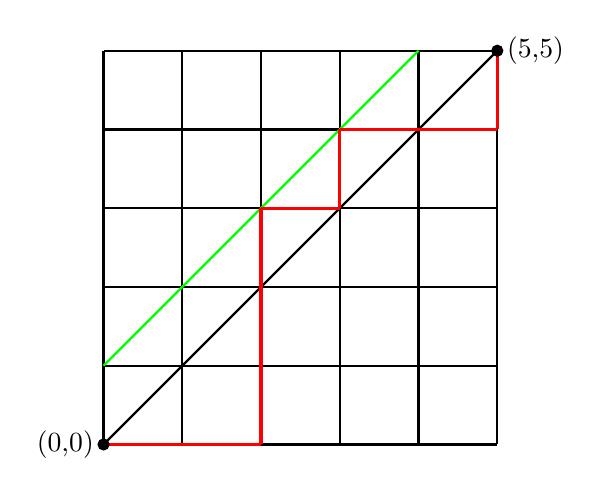
\begin{tikzpicture}
        \draw[black, thick] (0,0) -- (5,0);
        \draw[black, thick] (0,1) -- (5,1);
        \draw[black, thick] (0,2) -- (5,2);
        \draw[black, thick] (0,3) -- (5,3);
        \draw[black, thick] (0,4) -- (5,4);
        \draw[black, thick] (0,5) -- (5,5);
        \draw[black, thick] (0,0) -- (0,5);
        \draw[black, thick] (1,0) -- (1,5);
        \draw[black, thick] (2,0) -- (2,5);
        \draw[black, thick] (3,0) -- (3,5);
        \draw[black, thick] (4,0) -- (4,5);
        \draw[black, thick] (5,0) -- (5,5);
        \draw[green, thick] (0,1) -- (4,5);
        \draw[black, thick] (0,0) -- (5,5);
        \draw[red, very thick] (0,0) -- (2,0);
        \draw[red, very thick] (2,0) -- (2,3);
        \draw[red, very thick] (2,3) -- (3,3);
        \draw[red, very thick] (3,3) -- (3,4);
        \draw[red, very thick] (3,4) -- (5,4);
        \draw[red, very thick] (5,4) -- (5,5);
        \filldraw[black] (0,0) circle (2pt) node[anchor=east] {(0,0)};
        \filldraw[black] (5,5) circle (2pt) node[anchor=west] {(5,5)};
    \end{tikzpicture}
    \centering
    \caption{Fatal Line shown in green with a bad path shown in red}
    \label{fig:fatalLine}
\end{figure}
\begin{figure}[h!]
    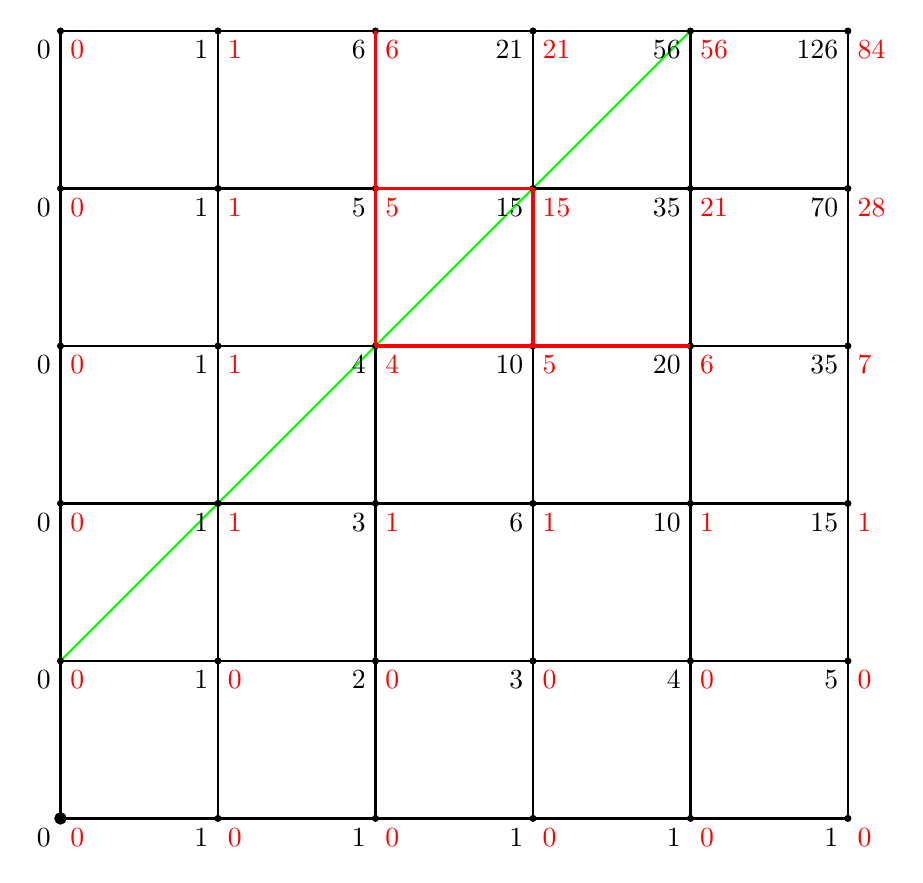
\begin{tikzpicture}
        \draw[black, thick] (0,0) -- (10,0);
        \draw[black, thick] (0,0) -- (0,10);
        \draw[black, thick] (0,10) -- (10,10);
        \draw[black, thick] (10,0) -- (10,10);
        \draw[black, thick] (2,0) -- (2,10);
        \draw[black, thick] (4,0) -- (4,10);
        \draw[black, thick] (6,0) -- (6,10);
        \draw[black, thick] (8,0) -- (8,10);
        \draw[black, thick] (0,2) -- (10,2);
        \draw[black, thick] (0,4) -- (10,4);
        \draw[black, thick] (0,6) -- (10,6);
        \draw[black, thick] (0,8) -- (10,8);
        \draw[green, thick] (0,2) -- (8,10);
        \filldraw[black] (0,0) circle (2pt) node[anchor=north east] {0};
        \filldraw[black] (0,0) circle (2pt) node[anchor=north west, text = red] {0};
        \filldraw[black] (2,0) circle (1pt) node[anchor=north east] {1};
        \filldraw[black] (2,0) circle (1pt) node[anchor=north west, text = red] {0};
        \filldraw[black] (4,0) circle (1pt) node[anchor=north east] {1};
        \filldraw[black] (4,0) circle (1pt) node[anchor=north west, text = red] {0};
        \filldraw[black] (6,0) circle (1pt) node[anchor=north east] {1};
        \filldraw[black] (6,0) circle (1pt) node[anchor=north west, text = red] {0};
        \filldraw[black] (8,0) circle (1pt) node[anchor=north east] {1};
        \filldraw[black] (8,0) circle (1pt) node[anchor=north west, text = red] {0};
        \filldraw[black] (10,0) circle (1pt) node[anchor=north east] {1};
        \filldraw[black] (10,0) circle (1pt) node[anchor=north west, text = red] {0}; \filldraw[black] (0,2) circle (1pt) node[anchor=north east] {0};
        \filldraw[black] (0,2) circle (1pt) node[anchor=north west, text = red] {0};
        \filldraw[black] (2,2) circle (1pt) node[anchor=north east] {1};
        \filldraw[black] (2,2) circle (1pt) node[anchor=north west, text = red] {0};
        \filldraw[black] (4,2) circle (1pt) node[anchor=north east] {2};
        \filldraw[black] (4,2) circle (1pt) node[anchor=north west, text = red] {0};
        \filldraw[black] (6,2) circle (1pt) node[anchor=north east] {3};
        \filldraw[black] (6,2) circle (1pt) node[anchor=north west, text = red] {0};
        \filldraw[black] (8,2) circle (1pt) node[anchor=north east] {4};
        \filldraw[black] (8,2) circle (1pt) node[anchor=north west, text = red] {0};
        \filldraw[black] (10,2) circle (1pt) node[anchor=north east] {5};
        \filldraw[black] (10,2) circle (1pt) node[anchor=north west, text = red] {0};
        \filldraw[black] (0,4) circle (1pt) node[anchor=north east] {0};
        \filldraw[black] (0,4) circle (1pt) node[anchor=north west, text = red] {0}; \filldraw[black] (2,4) circle (1pt) node[anchor=north east] {1};
        \filldraw[black] (2,4) circle (1pt) node[anchor=north west, text = red] {1};
        \filldraw[black] (4,4) circle (1pt) node[anchor=north east] {3};
        \filldraw[black] (4,4) circle (1pt) node[anchor=north west, text = red] {1};
        \filldraw[black] (6,4) circle (1pt) node[anchor=north east] {6};
        \filldraw[black] (6,4) circle (1pt) node[anchor=north west, text = red] {1};
        \filldraw[black] (8,4) circle (1pt) node[anchor=north east] {10};
        \filldraw[black] (8,4) circle (1pt) node[anchor=north west, text = red] {1};
        \filldraw[black] (10,4) circle (1pt) node[anchor=north east] {15};
        \filldraw[black] (10,4) circle (1pt) node[anchor=north west, text = red] {1};
        \filldraw[black] (0,6) circle (1pt) node[anchor=north east] {0};
        \filldraw[black] (0,6) circle (1pt) node[anchor=north west, text = red] {0}; \filldraw[black] (2,6) circle (1pt) node[anchor=north east] {1};
        \filldraw[black] (2,6) circle (1pt) node[anchor=north west, text = red] {1};
        \filldraw[black] (4,6) circle (1pt) node[anchor=north east] {4};
        \filldraw[black] (4,6) circle (1pt) node[anchor=north west, text = red] {4};
        \filldraw[black] (6,6) circle (1pt) node[anchor=north east] {10};
        \filldraw[black] (6,6) circle (1pt) node[anchor=north west, text = red] {5};
        \filldraw[black] (8,6) circle (1pt) node[anchor=north east] {20};
        \filldraw[black] (8,6) circle (1pt) node[anchor=north west, text = red] {6};
        \filldraw[black] (10,6) circle (1pt) node[anchor=north east] {35};
        \filldraw[black] (10,6) circle (1pt) node[anchor=north west, text = red] {7};
        \filldraw[black] (0,8) circle (1pt) node[anchor=north east] {0};
        \filldraw[black] (0,8) circle (1pt) node[anchor=north west, text = red] {0}; \filldraw[black] (2,8) circle (1pt) node[anchor=north east] {1};
        \filldraw[black] (2,8) circle (1pt) node[anchor=north west, text = red] {1};
        \filldraw[black] (4,8) circle (1pt) node[anchor=north east] {5};
        \filldraw[black] (4,8) circle (1pt) node[anchor=north west, text = red] {5};
        \filldraw[black] (6,8) circle (1pt) node[anchor=north east] {15};
        \filldraw[black] (6,8) circle (1pt) node[anchor=north west, text = red] {15};
        \filldraw[black] (8,8) circle (1pt) node[anchor=north east] {35};
        \filldraw[black] (8,8) circle (1pt) node[anchor=north west, text = red] {21};
        \filldraw[black] (10,8) circle (1pt) node[anchor=north east] {70};
        \filldraw[black] (10,8) circle (1pt) node[anchor=north west, text = red] {28};
        \filldraw[black] (0,10) circle (1pt) node[anchor=north east] {0};
        \filldraw[black] (0,10) circle (1pt) node[anchor=north west, text = red] {0}; \filldraw[black] (2,10) circle (1pt) node[anchor=north east] {1};
        \filldraw[black] (2,10) circle (1pt) node[anchor=north west, text = red] {1};
        \filldraw[black] (4,10) circle (1pt) node[anchor=north east] {6};
        \filldraw[black] (4,10) circle (1pt) node[anchor=north west, text = red] {6};
        \filldraw[black] (6,10) circle (1pt) node[anchor=north east] {21};
        \filldraw[black] (6,10) circle (1pt) node[anchor=north west, text = red] {21};
        \filldraw[black] (8,10) circle (1pt) node[anchor=north east] {56};
        \filldraw[black] (8,10) circle (1pt) node[anchor=north west, text = red] {56};
        \filldraw[black] (10,10) circle (1pt) node[anchor=north east] {126};
        \filldraw[black] (10,10) circle (1pt) node[anchor=north west, text = red] {84};
        
        \draw[red, very thick] (4,6) -- (8,6);
        \draw[red, very thick] (6,6) -- (6,8);
        \draw[red, very thick] (4,6) -- (4,10);
        \draw[red, very thick] (4,8) -- (6,8);
    \end{tikzpicture}
    \centering
    \caption{The number of paths to each point from (1,0) written in black and the number of bad paths is written in red. Also example of symmetry of a bad path which passes through (2,3) in red showing all possible 2 step combinations.}
    \label{fig:countingPaths}
\end{figure}

\newpage

\begin{theorem}\label{thm:final}
    The number of good paths from $(0,0)$ to $(n,m)$ is equal to
    \begin{equation}
        \binom{n+m-1}{n-1}-\binom{n+m-1}{n+1}.
    \end{equation}
\end{theorem}
\begin{proof}
    Using the equation in Lemma \ref{lem:goodPathEq}: $g = p - b$ and the equations for $p$ and $b$ defined in Equation \ref{eq:modifiedTotal} and Lemma \ref{lem:badPathEq} relatively we have
    \begin{align*}
        p &= \binom{n+m-1}{n-1}\\
        b &= \binom{n+m-1}{n+1}.
    \end{align*}
    Combining the equations, we get 
    \begin{align*}
        g &= \binom{n+m-1}{n-1}-\binom{n+m-1}{n+1}\\
    \end{align*}
    completing our proof.
\end{proof}

\begin{corollary}
    The number of good paths from $(0,0)$ to $(n,n)$ is equal to
    \begin{equation}
        \frac{1}{n+1}\binom{2n}{n}
    \end{equation}
\end{corollary}
\begin{proof}
    Let $n=m$, then we have
    \begin{align*}
        g &= \binom{2n-1}{n-1} - \binom{2n-1}{n+1}\\
        &= \frac{(2n-1)!}{(n-1)!(n)!} - \frac{(2n-1)!}{(n-2)!(n+1)!}\\
        &= \left[1-\frac{n-1}{n+1}\right]\frac{(2n-1)!}{(n-1)!(n)!}\\
        &= \frac{2}{n+1}\binom{2n-1}{n-1}\\
        &= \frac{1}{n+1}\binom{2n}{n}.
    \end{align*}
\end{proof}

\begin{corollary}
    The $n$th Catalan Number can be calculated by Equation 3
\end{corollary}
\end{document}